\chapter{Technologies}\label{ch:technologies}
With Solidity\footnote{https://github.com/ethereum/solidity}we implement the \ac{sc} which will run on the Ethereum blockchain. For our front-end we choose using React\footnote{https://reactjs.org/}, which is a JavaScript library for building user interfaces. The interaction of the front-end application with our \ac{sc} is provided through Web3.js\footnote{https://web3js.readthedocs.io/en/1.0/} and MetaMask\footnote{https://metamask.io/}. Furthermore, the application provides also the possibility to interact with a localhost provider using Ganache\footnote{http://truffleframework.com/ganache/} as Ethereum node.
\begin{figure}[ht]
	\begin{center}
		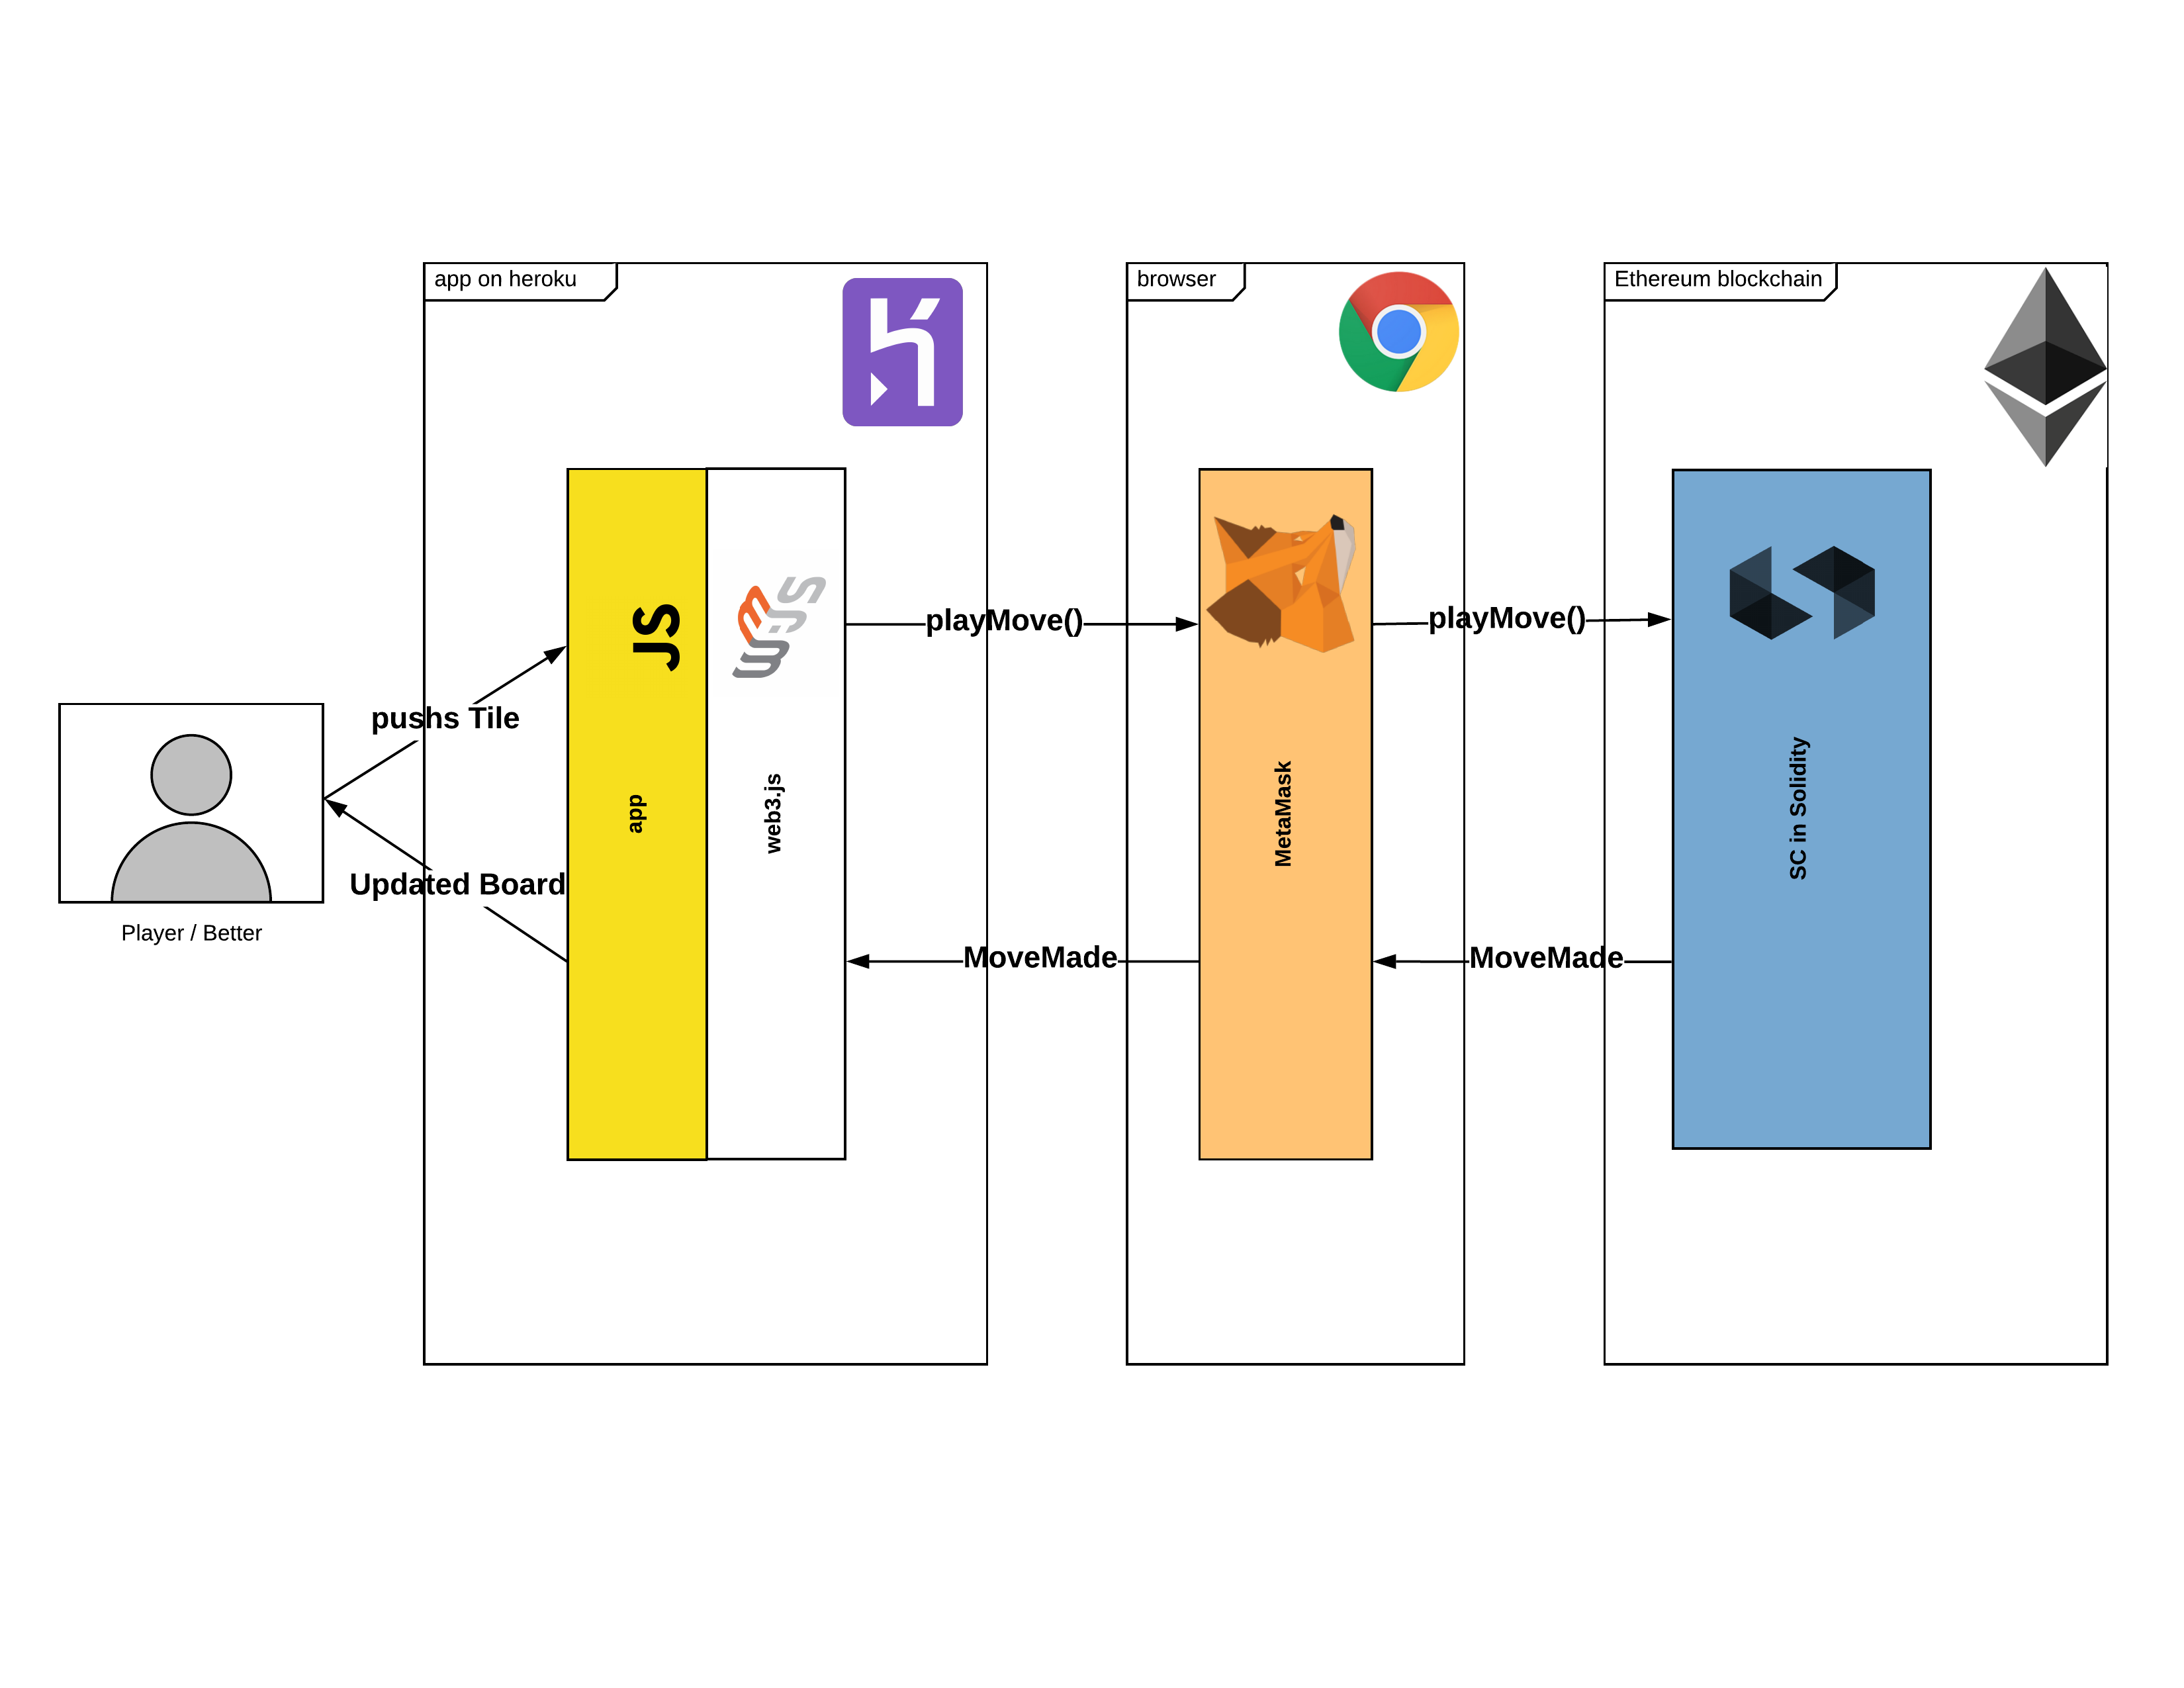
\includegraphics[scale=0.4]{res/project_structure}
	\end{center}
	\caption{The interconnection of the different technologies}
	\label{fig:interconnection}
\end{figure}\newpage
\noindent Figure \ref{fig:interconnection} shows the project structure and the interaction between these different systems by the example of an Player choosing a tile on the board.
The web-application is running on the Heroku Platform\footnote{https://www.heroku.com/}. Through the browser and MetaMask a User can get verified by its Ethereum-account and pay the requested amount of gas in order to run functionalities on the Ethereum \ac{sc}. The \ac{sc} itself runs on an blockchain, which can be either a private or the Ropsten Testnet\footnote{https://ropsten.etherscan.io/}.

